\documentclass[11pt,a4paper,twocolumn]{article}

\usepackage[margin=2cm]{geometry}
\usepackage{mathptmx}         
\usepackage{booktabs}
\usepackage{amsmath}
\usepackage{url}
\usepackage{graphicx}

\linespread{1.0}
\setlength{\parskip}{4pt}
\setlength{\parindent}{0pt}
\setlength{\columnsep}{20pt}




\title{\textbf{Individual Reflection Report}\\[4pt]
\large AI and Text Analytics Coursework -- Spring 2026\\
University of Bristol\\
Team 16, Task 1: PubMedQA Biomedical Question Answering}
\author{Peidong Wang\\
\texttt{hz25950@bristol.ac.uk}}
\date{\today}


\begin{document}
\maketitle

\section{Contributions Summary}

I volunteered to lead the \textbf{text-representation axis} (Axis 1) because I wanted to understand, from first principles, how much the choice of representation---not the classifier---drives performance on a biomedical reasoning task. My strategy was deliberately incremental: start with a transparent sparse baseline, then escalate to frozen contextual embeddings, and finally to full fine-tuning. I expected each step to yield clear gains; as I discuss in Section~2, the reality was more nuanced and, at times, humbling.

My concrete contributions were:

\begin{enumerate}
  \item \textbf{TF-IDF + LR Baselines (A1a/b/c):} implemented three input variants (Q, Q+Ctx, Q+Ctx+Ans\footnote{%
    \textbf{Ans} refers to the long-answer field provided in PubMedQA annotations---a human-written passage that directly explains the reasoning behind the label.
    In real-world deployment this field would not be available at inference time, making Q+Ctx+Ans an \emph{oracle} configuration.
    It is included here solely to probe the model's capability upper bound and to verify that the pipeline can correctly learn from rich evidence when that evidence is explicitly provided.}) to establish performance ceilings for sparse representations (\texttt{baseline\_lr\_group.py}).
  \item \textbf{BioBERT Embeddings + LR:} extracted frozen representations from \texttt{biobert-v1.2} for linear classification (A1d).
  \item \textbf{BioBERT Fine-tuning (Q+Ctx):} adapted the full model (\texttt{modeling\_biobert\_ft\_on\_q\_ctx.py}) with weighted cross-entropy (A1e).
  \item \textbf{BioBERT Fine-tuning (Q+Ctx+Ans):} extended fine-tuning to include long answers (\texttt{modeling\_biobert\_ft\_on\_q\_ctx\_ans.py}), probing the impact of input richness (A1f).
\end{enumerate}

Additionally, I implemented a custom data-splitting script (\texttt{data\_splitter.py}) to cross-verify the stratified 500/500 split and 10-fold CV protocol---partly out of caution, and partly because I wanted independent confidence in the preprocessing before building experiments on top of it.

\medskip
\begin{figure}[h]
  \centering
  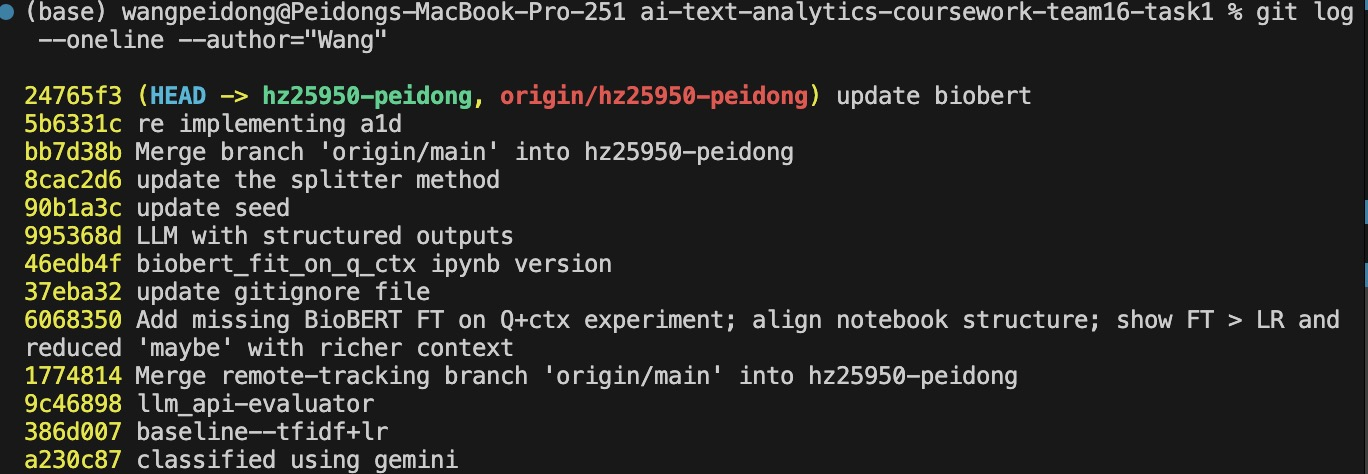
\includegraphics[width=\linewidth]{git_log_by_wang.jpg}
  \caption*{\textit{Figure 1: GitHub commit activity -- commits attributed to Peidong Wang.}}
\end{figure}


\section{Technical Understanding}

\subsection*{2a. Technical Challenge: Input Composition and Class Imbalance}

PubMedQA presents two interacting challenges: extreme class imbalance (\emph{maybe} is only 11\%) and the conditional utility of the long answer field. 
For the baseline, I addressed imbalance using \texttt{class\_weight="balanced"}. For BioBERT, I implemented a \texttt{WeightedTrainer} to inject per-class weights into \texttt{CrossEntropyLoss}, ensuring methodological consistency.

Crucially, my TF-IDF baselines (A1a/b/c) exhibited a performance plateau (macro-F1 $\sim 0.35$) regardless of input composition, suggesting that sparse representations cannot leverage extended context. In contrast, while BioBERT on Q+Ctx alone (A1e, $0.294$) underperformed the baseline, adding the long-answer channel (A1f) lifted macro-F1 to $0.466$. While this field acts as an "oracle" unavailable in practical deployment, the A1f experiment was vital to confirm the model's upper-bound capacity.

\subsection*{2b. Impact on Group Results}

My experiments (A1a--f) established the "Axis-1" narrative in the group report. While frozen BioBERT embeddings (A1d) improved \emph{maybe}-class recovery ($0.057 \to 0.172$), the A1e-vs-A1f comparison provided our central empirical finding: adding the long answer yields a $+0.17$ macro-F1 gain for transformers, a trend not observed in TF-IDF. This finding motivated the team's final transition to PubMedBERT (A1g), which achieved our peak result of $0.604$.

\subsection*{2c. Reflection and Future Work}

Beyond our official axes, I exploratory-tested a zero-shot LLM (Gemini API), achieving a macro-F1 of $0.611$—surpassing our fine-tuned models. This suggests that future work should prioritize generative reasoning. Specifically, techniques such as \textbf{Chain-of-Thought (CoT)} or \textbf{step-wise verification} could further improve the detection of inconclusive evidence by forcing the model to explicitly assess evidence-sufficiency before label assignment, addressing the core bottleneck of the \emph{maybe} class.

\medskip
\noindent\textbf{Representation Quality Ablation: Context Window in A1d.}
A key question in Axis 1 is whether \emph{frozen} BioBERT representations genuinely encode biomedical evidence, or whether their performance ceiling is an artefact of how the encoder was configured. To probe this, I conducted an ablation on the \textbf{effective context window} used during embedding extraction in A1d. The original run relied on \texttt{SentenceTransformer}'s default of \textbf{100 tokens}, which is insufficient to cover the vast majority of Q+Context inputs in PubMedQA, meaning that most of the medical evidence passage never reached the encoder.

Re-implementing A1d with \texttt{AutoModel}, explicit \texttt{max\_length=384}, and mean-pooling (\texttt{modeling\_biobert\_lr.py \& modeling\_biobert\_ft\_on\_q\_ctx.ipynb}) raised the test macro-F1 from $0.353$ to $0.419$ ($+18.7\%$), with \emph{maybe}-class F1 improving from $0.172$ to $0.180$. This ablation demonstrates that \textbf{the quality of a frozen representation is tightly coupled to how much context the encoder can read}: the A1d result reported in the group submission was limited by the encoding window, not by the expressiveness of BioBERT itself. This finding is squarely within Axis 1's scope---it concerns the fidelity of text representations, independent of classifier-level tuning explored under Axis 2.


\section{Teamwork}


The team coordinated through a shared \textbf{GitHub repository}
(\texttt{ai-text-analytics-coursework-team16-task1}), using personal branches. Discussing in a group chat on \textbf{WhatsApp}.  A shared \textbf{Jira board} tracked task
ownership, deadlines, and blockers; weekly online check-ins and meetings via
\textbf{Microsoft Teams} kept everyone aligned.

Role assignments were as follows:

\begin{itemize}
  \item \textbf{Abdullah} -- data loading, preprocessing, label encoding, text
        input creation, train-test split, and 10-fold CV setup; dataset sanity
        checks, label-distribution and split-count verification, and export of
        the final cleaned dataset and split-summary tables.
  \item \textbf{Peidong Wang} -- TF-IDF + LR baseline, BioBERT embeddings + LR,
        and BioBERT end-to-end fine-tuning (Axis 1: text representation).
  \item \textbf{Zhengjie} -- classical Axis 2 models: tuned LR, calibrated SVM,
        Multinomial NB, SMOTE + LR, and soft-voting ensemble.
  \item \textbf{Abhigyan} -- error analysis: confusion matrix checks,
        misclassified-example inspection, cross-model comparison notes, and
        result verification.
  \item \textbf{Tanishk} -- advanced transformer and maybe-class models
        (PubMedBERT, LoRA, zero-shot BART, focal loss, threshold tuning, ordinal
        loss, hierarchical classifier); final integration, tables, graphs, result
        export, and notebook cleanup.
\end{itemize}

Every member participated in at least one evaluation sprint, and all
results were cross-checked to guarantee reproducibility.  A fixed random seed (\texttt{SEED = 42}) was
adopted collectively across all scripts to ensure experimental consistency.

\end{document}
